\chapter{Fundamentação Teórica}

\label{cap:2}

Neste capítulo serão abordados fundamentos e conceitos relevantes para este trabalho e apresentados trabalhos relacionados. São apresentados os conceitos de memória virtual e TLB. Em seguida, uma breve explicação sobre como ocorrem as falhas causadas por interferências externas. Então, uma seção demonstra quais problemas essas falhas podem causar às TLBs. Também é importante saber como se faz o cálculo da paridade simples e do código Hamming. Por fim, um revisão de trabalhos relacionados é apresentada, comentando sobre códigos de proteção à sistemas de memória e TLBs.

\section{Memória virtual}

Quando um sistema de memória utiliza memória virtual, o tamanho total de um
programa a ser executado podem ser
superiores à quantidade de memória física disponível para ele. O sistema operacional
armazena as partes ativas do programa na RAM e deixa o restante em disco. Quando o
programa entra em estado de execução, as páginas virtuais são transferidas do disco para a
memória principal.

Nessa técnica, o número da página virtual identifica a página virtual que é
associada ao endereço físico, funcionando como um índice na tabela de páginas. A Figura \ref{fig:memory} é uma representação desse esquema. Além dos endereços, a tabela de páginas possui outras informações, como o bit de validade, que indica se
uma página está ou não na memória principal. Se o bit tem valor 0, isto indica que a página
virtual não está na RAM, mas se o valor do bit é igual a 1, a página está na memória
principal \cite{Tannenbaum}.

\begin{figure}[ht]
    \centering
    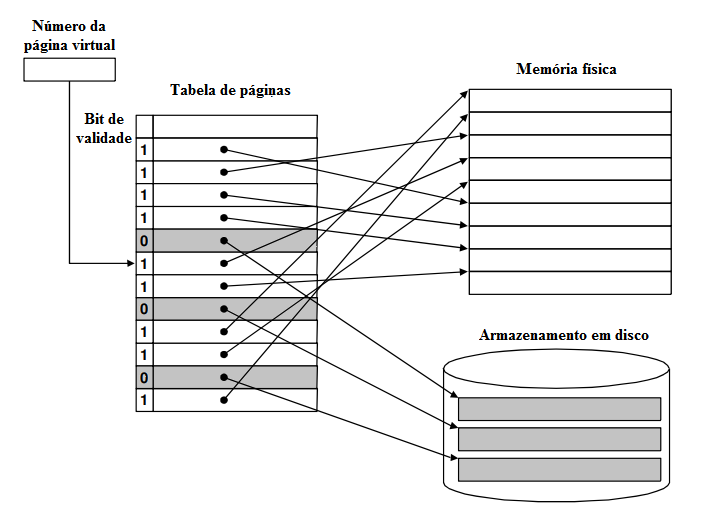
\includegraphics[scale=0.5]{figuras/memoria virtual.PNG}
    \caption{Esquema explicativo da memória virtual}{Fonte: adaptação de \cite{Tannenbaum}}
    \label{fig:memory}
\end{figure}

Sempre que um programa faz referência a um
endereço virtual, o MMU localiza na tabela de páginas o endereço físico correspondente.
Caso a página não esteja na memória, dizemos que ocorreu uma falta de página. Se a RAM
já estiver cheia, o sistema operacional se utiliza de algoritmos de substituição de páginas
para transferir páginas da memória principal para o disco, em seguida busca a página
desejada no disco e transfere para a memória principal.

\section{CAM}

Uma memória do tipo CAM usa um mecanismo de pesquisa e busca de endereços para verificar se as palavras buscadas estão armazenadas na memória. A Figura \ref{fig:cam} mostra como a CAM funciona. Quando uma palavra é buscada, a CAM precisa verificar a compatibilidade de cada bit da palavra com os bits armazenados em suas células de memória. Na entrada de cada célula de memória há um elemento de comparação, que assume os valores zero ou um de acordo com a combinação ou não do bit buscado com o bit armazenado. Como as células estão conectadas em paralelo, o impulso elétrico com os valores buscados chega em todas as células ao mesmo tempo. Então, um elemento chamado \textit{match line} verifica se houve combinação em todos os bits de cada linha, ou seja, se o valor  assumido das combinações foi um e o circuito fecha naquela linha. Se houver, significa que o endereço buscado foi encontrado \cite{maestro2013soft}.

\begin{figure}[ht]
    \centering
    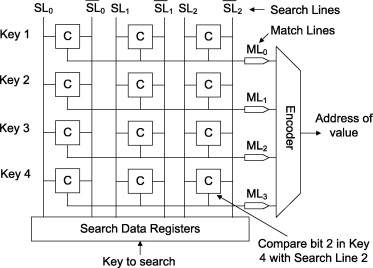
\includegraphics[scale=0.7]{figuras/cam.png}
    \caption{Arquitetura de uma CAM}{Fonte: \cite{maestro2013soft}}
    \label{fig:cam}
\end{figure}

Uma TLB é uma cache normalmente implementada com a arquitetura de uma CAM. Ela serve para acelerar o processo de tradução entre endereços físicos e virtuais. Na seção a seguir, ela será melhor abordada.

\section{TLB}
Nos sistemas de memória que utilizam paginação, as tabelas de páginas são
mantidas dentro da memória principal, devido a suas grandes dimensões, o que interfere
diretamente no desempenho do sistema. A maioria dos programas tende a referenciar mais vezes o mesmo pequeno grupo de páginas virtuais, que vai mudando ao longo da execução.
Sabendo disto, foi criada uma cache que se localiza dentro do MMU, portanto, mais perto
do gerenciador de memória, que armazena apenas as páginas mais referenciadas. A essa
cache foi dada o nome de \textit{translation lookaside buffer}(TLB). A Figura \ref{fig:arq} é uma representação dessa organização. O endereço virtual é buscado na TLB. Caso esteja, acontece um TLB \textit{hit}, dispensando o acesso à tabela de páginas e acelerando o processo de tradução. Caso não esteja na cache, acontece um TLB \textit{miss} e a tabela de páginas é consultada. 

\begin{figure}[ht]
\centering
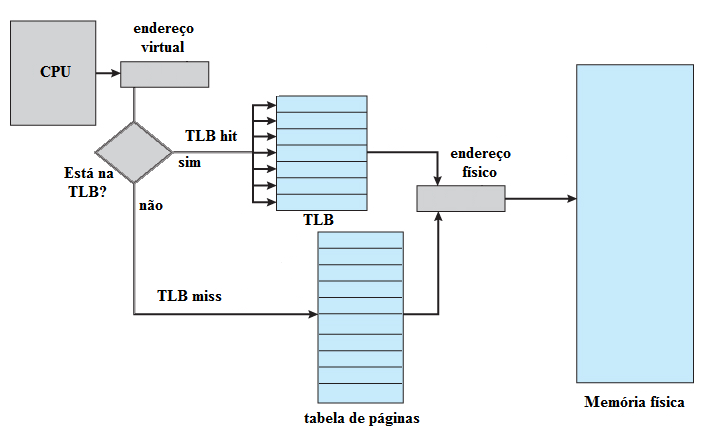
\includegraphics[scale=0.7]{figuras/tlbesquema.png}
\caption{Representação da arquitetura do processo de tradução}{Fonte: próprio autor}
\label{fig:arq}
\end{figure}

O fluxo desse funcionamento pode ser conferido na Figura \ref{fig:fluxo}. No processo de tradução de um endereço virtual, o sistema operacional verifica
primeiro a TLB. Se ocorrer uma TLB \textit{hit}, o processador acessa o endereço físico. Se ocorrer uma TLB \textit{miss}, será verificado se a página está na memória principal. Se sim, a tradução de seu endereço virtual é carregada na cache e o endereço é traduzido. Por outro lado, se não estiver na memória principal, o MMU faz uma chamada de sistema e indica
que houve falta de página. A página desejada precisa então ser carregada do disco para a
memória e se esta estive cheia, uma rotina de substituição de página é realizada. Em seguida, a tabela de páginas deve ser atualizada e os dados enviados para a TLB. Sempre
que há essa troca de contexto, a TLB deve ser reinicializada com as informações da nova
tabela de páginas. 
Tanto o processo de tratar falta de paginação quanto o de carregar na TLB as
informações novas, acabam sendo demorados, e influenciam no desempenho do sistema.

\begin{figure}[ht]
\centering
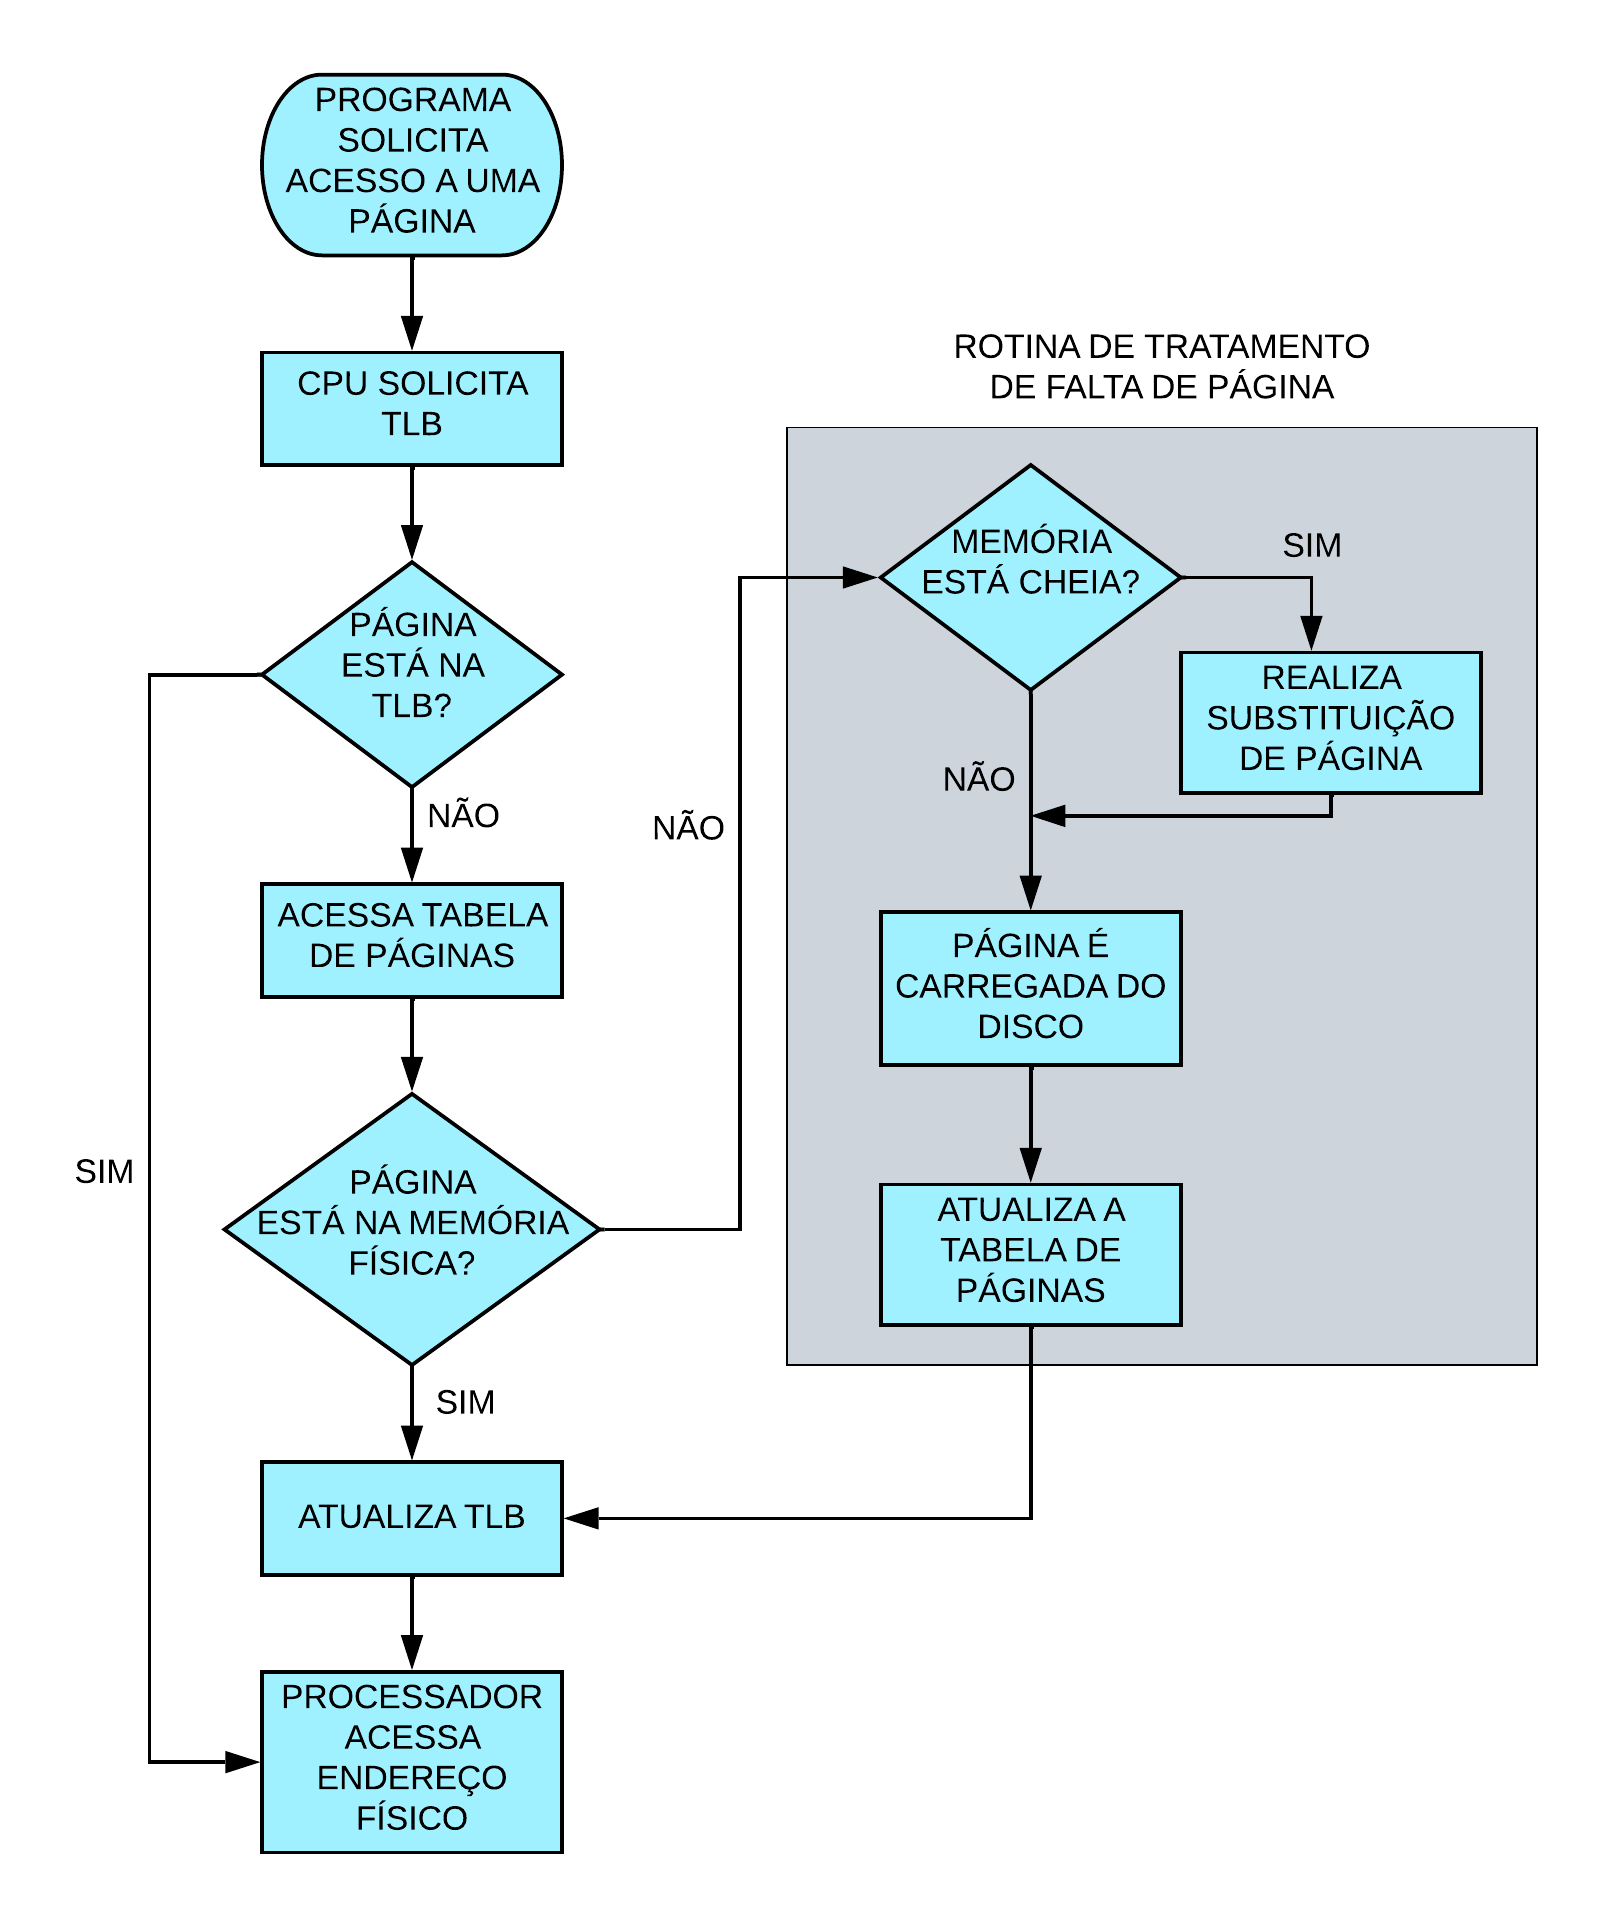
\includegraphics[scale=0.8]{figuras/fluxogramatlb.png}
\caption{Fluxograma do processo de tradução}{Fonte: próprio autor}
\label{fig:fluxo}
\end{figure}

\subsection{TLB \textit{miss} e TLB \textit{hit}}

A Figura \ref{fig:hit&miss} exemplificar melhor o que seria a TLB \textit{miss} e a TLB \textit{hit}, considerando um exemplo binário de endereço virtual com 8 bits: "11011001", que é buscado em uma TLB simples de 4 linhas. Nessa TLB estão os endereços "11011011", "11011010", "11011101", "11011000". São todos endereços próximos, mas nenhum igual ao requisitado. Acontece uma TLB \textit{miss} (a) e o processador busca o endereço na tabela de páginas. Se considerarmos que o endereço está na tabela de páginas, um algoritmo de substituição de páginas irá substituir um dos endereços que estavam na TLB anteriormente. No exemplo da figura, o endereço "11011011" foi substituído e a TLB foi atualizada com o endereço que estava sendo buscado. Se este mesmo endereço for buscado de novo, ele já está na TLB e acontece o \textit{hit} (b).

\begin{figure}[ht]
    \centering
      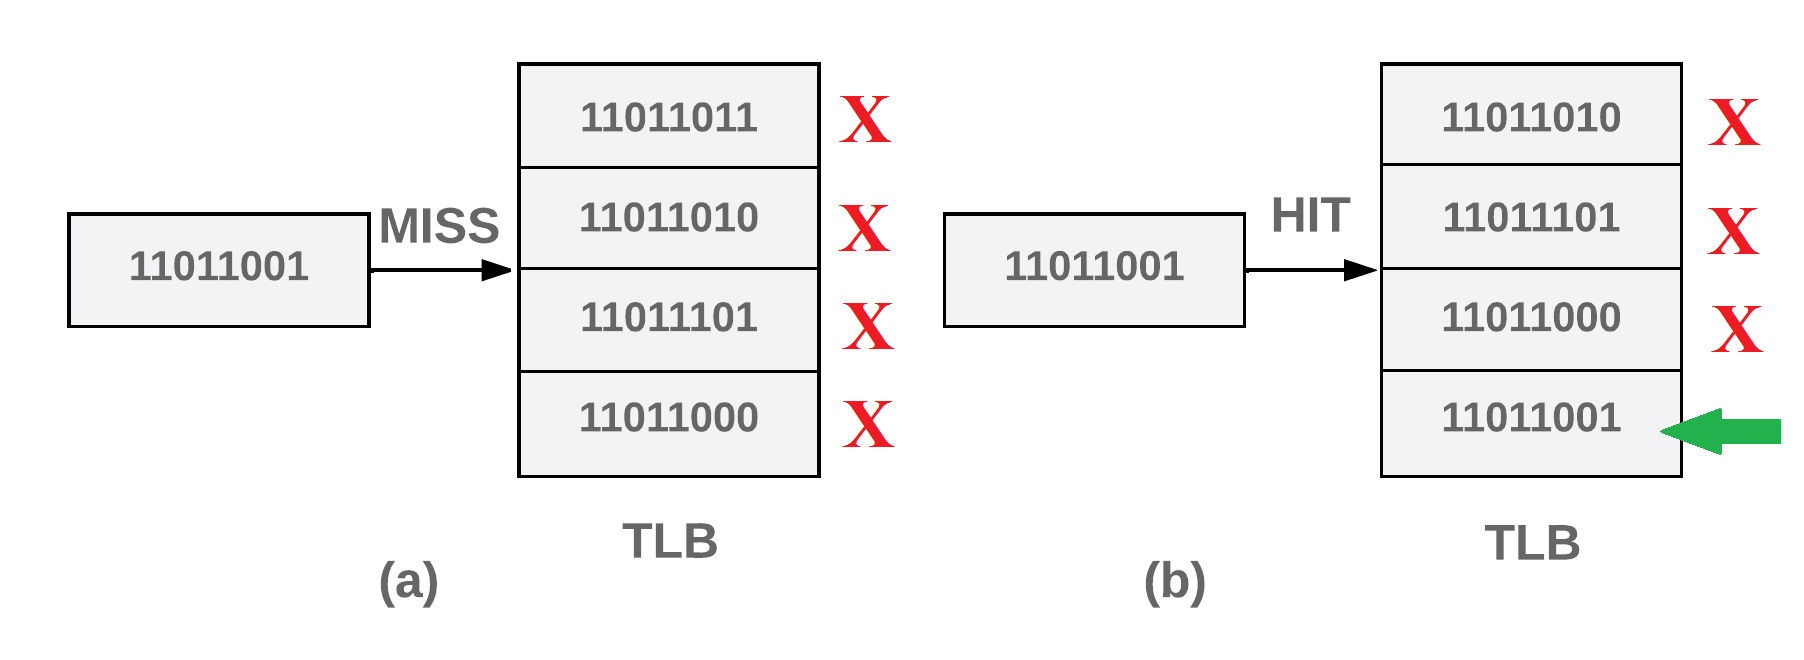
\includegraphics[scale=0.3]{figuras/hit&miss.png}
    \caption{Exemplo de TLB \textit{miss} (a) e TLB \textit{hit} (b)}{Fonte: próprio autor}
    \label{fig:hit&miss}
\end{figure}



\section{Falsos negativos e falsos positivos}

As entradas de uma TLB estão sujeitas a sofrerem com a ação de interferências externas, que podem alterar o valor do bit armazenado naquela célula de memória. Quando um erro atinge as entradas de uma TLB de instruções, podem ser produzidos dois tipos de falhas: falsos negativos e falsos positivos.

Falsos negativos acontecem quando os erros afetam os números das páginas
virtuais (NPVs) e o valor indicado pela TLB não corresponde mais ao valor original. Uma
falta de página é produzida e a nova informação deve ser recarregada da tabela de páginas da RAM. Na Figura \ref{fig:fneg}, inicialmente está representada uma TLB com alguns endereços de 8 bits (a). Em seguida, uma interferência atinge dois bits (b). Quando um um endereço é buscado pelo sistema, ele não coincide com os endereços na TLB (c). Neste caso, a TLB \textit{miss} resulta em uma rotina de tratamento de páginas e este processo pode atrapalhar o desempenho do sistema.

\begin{figure}[ht]
\centering
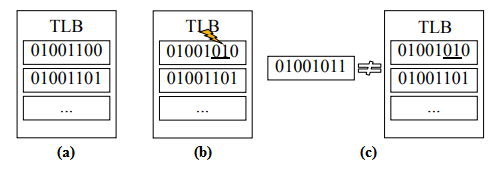
\includegraphics[scale=0.82]{figuras/FN_.PNG}
\caption{Falso negativo}{Fonte: próprio autor}
\label{fig:fneg}
\end{figure}

Por outro lado, no caso dos falsos positivos, o valor indicado pela TLB corresponde a uma página existente, no entanto, incorreta. Semelhante ao exemplo anterior, na Figura \ref{fig:fpos} tem-se a representação de um TLB (a), em que a falha também atinge dois bits (b). No entanto, dessa vez o endereço buscado coincide com o endereço após a alteração, gerando um falso positivo (c). Acontece um \textit{hit}, porém a tradução para endereço físico é errada. O número do endereço físico associado ao NPV é recuperado e uma instrução diferente da esperada é executada. Em casos extremos, isso pode causar falhas graves como congelamento do sistema ou até mesmo corrupção de dados. 

\begin{figure}[ht]
\centering
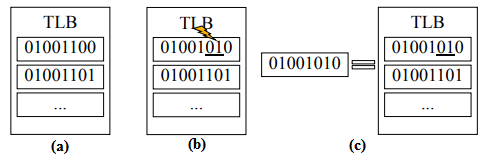
\includegraphics[scale=0.8]{figuras/FP_.PNG}
\caption{Falso positivo}{Fonte: próprio autor}
\label{fig:fpos}
\end{figure}

Considerando um exemplo semelhante ao visto na Figura \ref{fig:hit&miss} para melhor exemplificar estes conceitos, a Figura \ref{fig:fpex} representa um caso de falso positivo. Em (a) aconteceria um \textit{miss}, no entanto uma falha atinge o bit menos significativo do endereço "11011000", alternando seu valor para "11011001". Desse modo, em (b), a palavra buscada coincide com a que foi alterada. Como originalmente o endereço apontado era outro, a instrução errada vai ser executada.

\begin{figure}[ht]
    \centering
    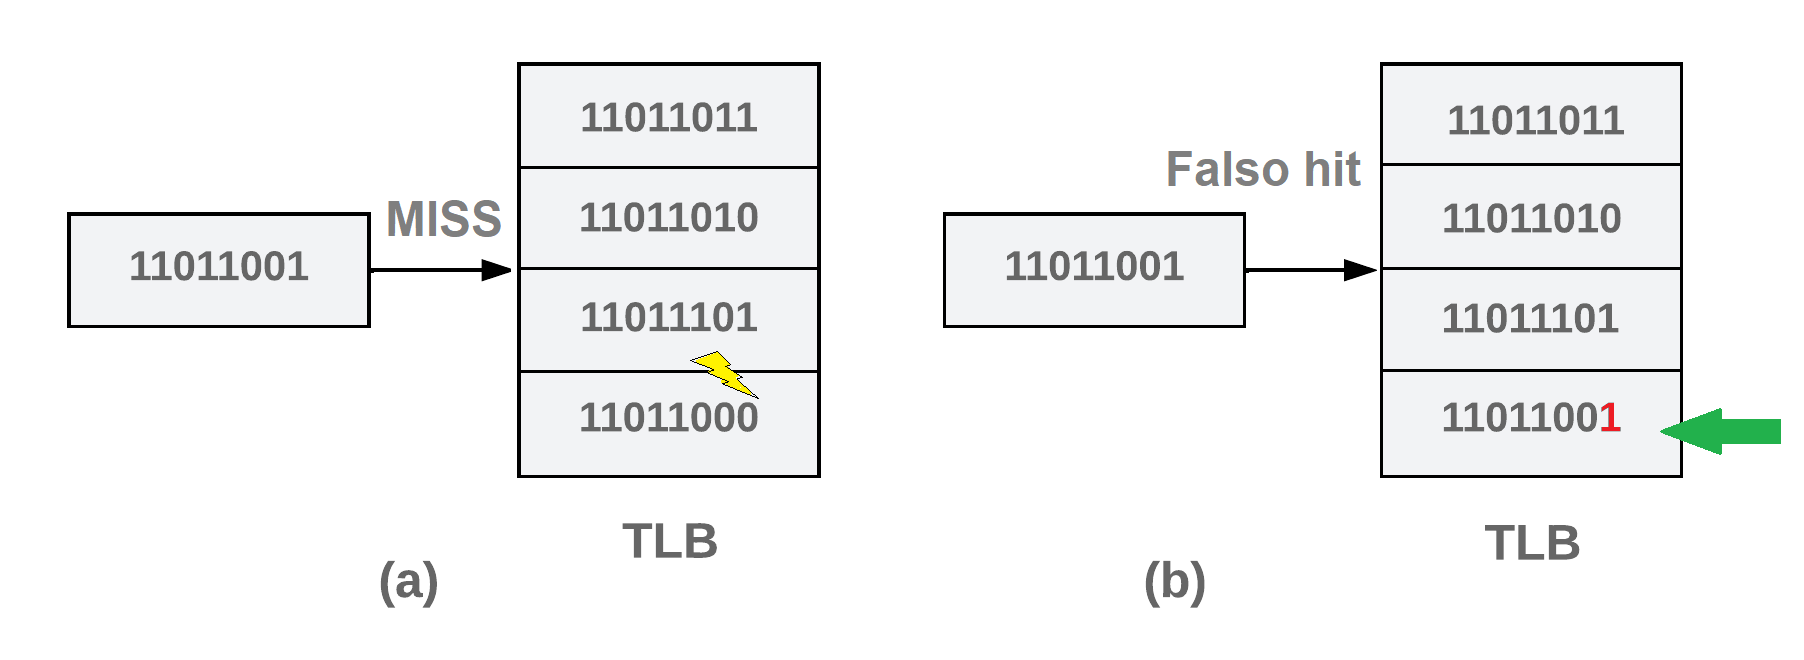
\includegraphics[scale=0.3]{modelo-dissertacao-ppgcc/figuras/FP.png}
    \caption{Exemplo de falso positivo}{Fonte:próprio autor}
    \label{fig:fpex}
\end{figure}

Do mesmo modo, a Figura \ref{fig:fnex} representa um exemplo de falso negativo. Considerando uma situação em que, em (a), haveria um \textit{hit}, já que existe coincidência entre a palavra buscada e um dos endereços da TLB. Se, nesse caso, uma falha atingisse o endereço "11011001" no "0" menos significativo, a palavra alterada seria "11011011". Assim, não há mais coincidência, logo a TLB indica uma \textit{miss}. O processo de tratamento de falta de página acontece sem necessidade, já que o endereço buscado já poderia ter sido apontado. Se recorrente, esse tipo de falha pode atrapalhar o desempenho do sistema.

\begin{figure}[ht]
    \centering
    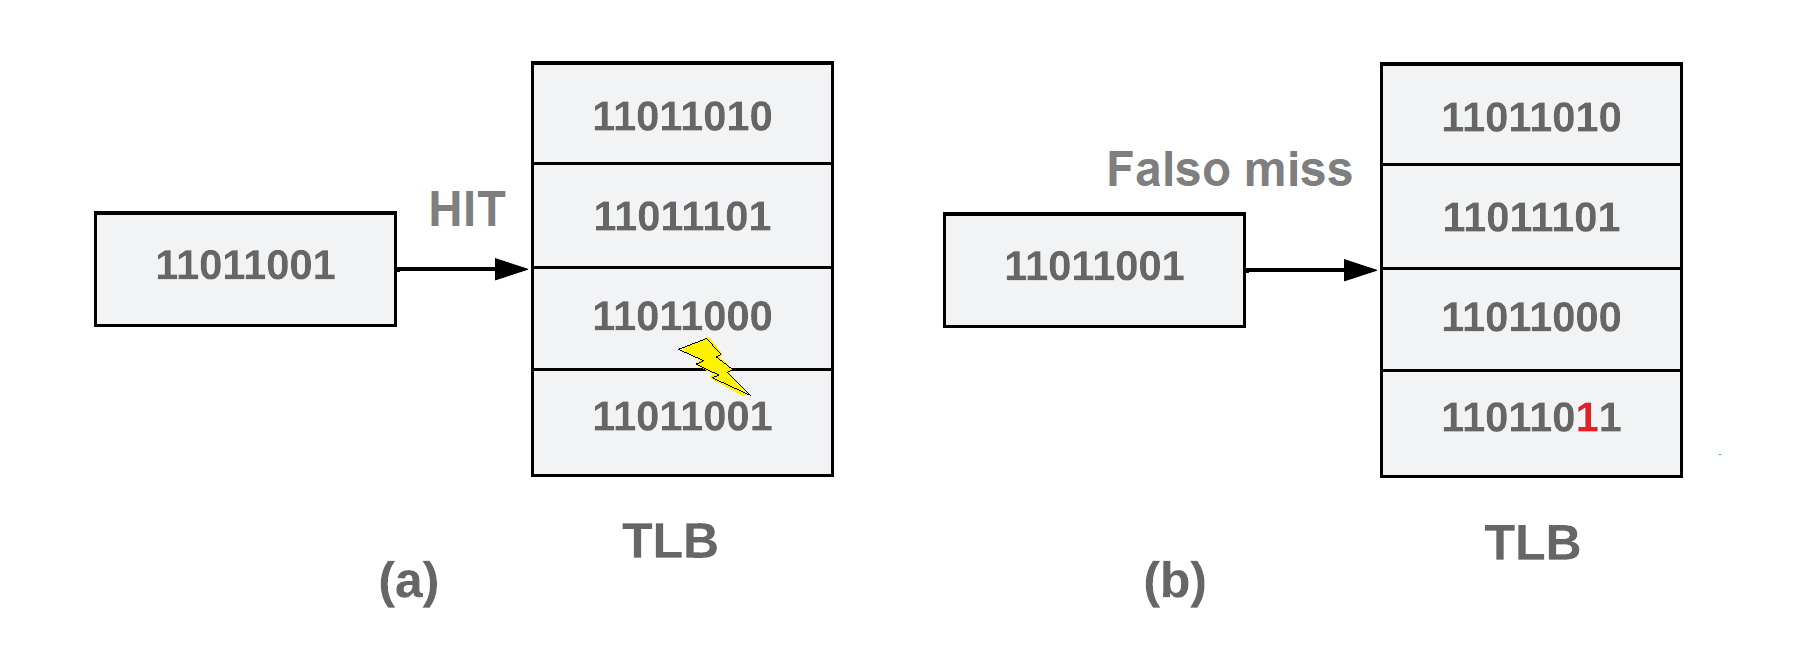
\includegraphics[scale=0.3]{modelo-dissertacao-ppgcc/figuras/FN.png}
    \caption{Exemplo de falso negativo}{Fonte:próprio autor}
    \label{fig:fnex}
\end{figure}

Os exemplos vistos mostram TLB pequenas e erros simples, mas essas falhas também acontecem em TLBs maiores e atingindo uma quantidade maior de bits. Os efeitos da radiação e outras interferências externas em circuitos cada vez mais integrados aumentam a possibilidade múltiplos bits atingidos.  

\section{A influência da radiação em dispositivos eletrônicos}

A radiação está presente em diversas formas e lugares, então dispositivos eletrônicos, mesmo em situações cotidianas, estão expostos a fatores que podem levá-los ao mau funcionamento. Em aplicações mais críticas, como as aplicações aeroespaciais, o sistema de memória está mais suscetível a interferências provenientes do ambiente, aumentando a ocorrência de MCUs \cite{varghese2013multiple}.

As junções de um transistor são muito sensíveis à radiação \cite{baumann2005soft}, então diversos eventos que acontecem à dispositivos orbitando a Terra podem alterar o estado de uma informação armazenada numa célula de memória ou durante uma transmissão de dados.

A figura a seguir mostra um exemplo de erro causado por interferências externas, apontando duas possíveis causas: uma queda de tensão ou causas ambientais como ondas eletromagnéticas \cite{vankeirsbilck2015integration}.

\begin{figure}[ht]
\centering
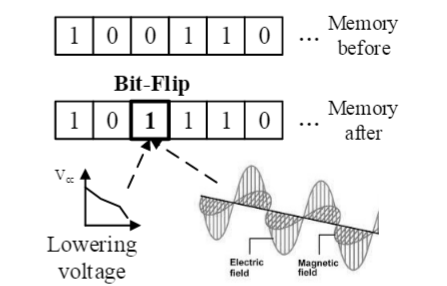
\includegraphics[scale=0.6]{figuras/error.PNG}
\caption{Exemplo de falha causada por interferências externas.}{Fonte: \cite{vankeirsbilck2015integration}}
\label{fig:error}
\end{figure}

\cite{slayman2005cache} disse que, em aplicações terrestres, a probabilidade de duas células de memória vizinhas serem afetadas por um erro durante um evento ionizante, é dez vezes menor que uma única célula. Enquanto \cite{seifert2008multi} mostraram que, em órbita, é muito mais provável a ocorrência de múltiplos erros. 

Os experimentos de \cite{satoh2000geometric} mostraram que as células afetadas são, na maioria das vezes, fisicamente próximas ou até mesmo adjacentes, após testes com sistemas de memória usando interferências externas espalhadas aleatoriamente pelas células. \cite{lawrence2008single} testaram sistemas de memórias para mostrar que single events upsets podem também afetar múltiplos bits, após ionização em diferentes aplicações.

Nesses cenários, códigos simples, como o cálculo de paridade e o código Hamming, não são o suficiente para minimizar os efeitos da radiação. Com isso, é necessário utilizar códigos mais robustos.

\section{Paridade}

Um dos métodos mais fáceis e mais utilizados para detecção de erros em sistemas de memória, é o cálculo da paridade. A codificação consiste em verificar a quantidade de bits em nível lógico alto e adicionar um bit com o valor da paridade. Normalmente as entradas de uma TLB já possuem um mecanismos de detecção de erros que utiliza o cálculo de um bit de paridade. Quando um erro é detectado, aquela entrada é invalidada e a TLB solicita novo envio \cite{griffith2005tlb}.

Existem dois tipos de paridade: 

\begin{itemize}
    \item paridade par: Quando um número binário (também chamado de palavra) possui um número par de 1's, então o bit de paridade será 0, para manter um número par de 1's. Desse modo, se o número de 1's é ímpar, então o bit de paridade será 1.
    \item paridade ímpar: Quando um número binário possui um número ímpar de 1's, então o bit de paridade será 0, para manter um número ímpar de 1's. Desse modo, se o número de 1's é par, então o bit de paridade será 1.
\end{itemize}

Para exemplificar isto, considerando a palavra 01100101, a quantidade de 1's nela é par. Neste caso, se a paridade for do tipo par, o bit de paridade será 0. Se a paridade for ímpar, então o bit de paridade será 1.

Essa operação pode ser representada por $\oplus$, que simboliza a porta lógica Ou-Exclusivo, ou apenas XOR. No caso do exemplo acima, utilizando paridade par, temos:
\begin{equation}
    0 \oplus 1 \oplus 1 \oplus 0 \oplus 0 \oplus 1 \oplus 0 \oplus 1 = 0
\end{equation}

Desse modo, o bit adicionado à palavra é 0, então a palavra codificada é 001100101, onde o 0 mais à esquerda é o bit de paridade (BP).
Se uma falha atinge uma célula de memória e um dos bits de nível lógico baixo muda seu valor de 0 para 1 (indicado abaixo em negrito), a nova quantidade de 1's agora é ímpar e o bit de paridade adicionado deveria ser 1.
\begin{equation}
    \textbf{1} \oplus 1 \oplus 1 \oplus 0 \oplus 0 \oplus 1 \oplus 0 \oplus 1 = 1
\end{equation}
    
O processador codifica a palavra como 111100101, sendo o 1 mais à esquerda o novo bit de paridade(BP'). A detecção de erro ocorre quando os dois bits de paridade são comparados.
\begin{equation}
    BP \oplus BP' = 0 \oplus 1 = 1
\end{equation}

Assim, é indicada a presença de erro na palavra armazenada.

Deste ponto em diante, sempre que for citado paridade neste trabalho, estará sendo considerada a paridade par.


\section{Código Hamming}

O matemático americano Richard Hamming criou em 1950 um código de detecção e correção que recebeu seu nome \cite{milies2009breve}. Até hoje, o código Hamming é bastante utilizado em diversas aplicações na computação, inclusive como base para outros códigos de correção de erro. O código permite não só detectar a presença de um erro, mas também a sua localização. Sabendo a posição do bit alterado na palavra, é possível corrigi-lo. Além disso, consegue detectar até dois bits com erros. Portanto, o Hamming é um código do tipo SEC-DED (Single Error Correction - Double Error Detection).

Como pode ser visto na Figura \ref{fig:hamming}, o código Hamming ocorre da seguinte maneira: os bits de redundância são adicionados intercalados aos bits da palavra original (a), e seus valores são calculados de uma forma específica (b). Por exemplo, o bit de paridade P1 é o resultado de D1 $\oplus$ D2 $\oplus$ D4.

\begin{figure}[ht]
    \centering
    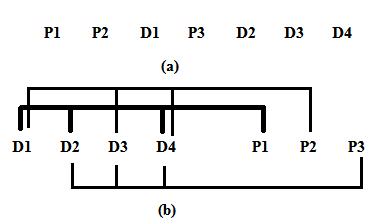
\includegraphics[scale=0.7]{figuras/hamming.png}
    \caption{Código Hamming, distribuição dos bits (a) e cálculo de paridades (b)}{Fonte: próprio autor}
    \label{fig:hamming}
\end{figure}

O número de bits de redundância depende do número de bits de dados, seguindo a equação 
\begin{equation}
    2^m-1=n
\end{equation}
em que m é o número de bits de redundância e n o número total de bits da palavra codificada.


\section{Trabalhos Relacionados}

A teoria moderna de códigos originou-se com o trabalho de Claude Shannon, que teve papel importante na base teórica do que hoje chamamos códigos corretores de erros \cite{meneghesso2012codigos}. A ideia central desses códigos usados em sistemas de memória é a adição de bits de redundância nos dados a serem transmitidos, codificando-os. Os receptores usam essas redundâncias para verificar a consistência da mensagem, podendo,
caso encontre erro, corrigi-lo por meio da decodificação.

Alguns dos códigos corretores de erros mais antigos são os da família Reed-Muller, desenvolvidos na década de 1950 e sendo utilizado em aplicações espaciais. Foi implementado nas sondas Mariner, que transmitiam fotos da superfície de Marte \cite{varghese2013multiple}.

Outro desses códigos capazes de lidar com MCUs em memórias é o código Matrix \cite{argyrides2007matrix}. Esse código associa o código de Hamming com paridade, codificando uma palavra em formato matricial. O Reed-Muller é mais robusto que o Matrix e apresenta taxa de correção maior, no entanto, os custos de implementação do Matrix são muito menores.

Outras formas de codificar palavras binárias vêm sendo propostas e estudadas nos últimos anos. A seguir serão apresentadas algumas delas.

\subsection{Códigos de correção de erros}

Usando conceitos de Hamming Estendido e paridade, o \textit{Column Line Code} (CLC) \cite{castro2016correction} é um código matricial que apresenta custo de implementação bem mais baixos que o Reed-Muller e taxas de correção maiores que o Matrix. A Figura \ref{fig:clc} mostra como se distribui os bits de redundância adicionados após a codificação do CLC. Na figura, C são os bits de dados, CB são calculados a partir do Hamming de cada linha de dados, Pa é o resultado do Hamming Estendido, e P são as paridades, calculadas para cada coluna. Posteriormente, \cite{silva2018extensible} apresenta uma versão melhorada do CLC, o CLC Estendido, que incrementa as capacidades de proteção do código.

\begin{figure}[ht]
    \centering
    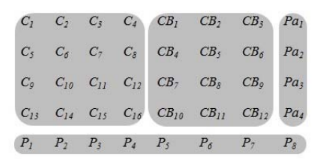
\includegraphics[scale=1]{figuras/clc.PNG}
    \caption{Codificação do CLC com 16 bits de entrada}{Fonte: \cite{castro2016correction}}
    \label{fig:clc}
\end{figure}

Numa nova melhoria do código, os autores  apresentam, o CLC-A, que fica alternando entre o CLC Padrão e o CLC Estendido de acordo com o tipo de erro detectado, e essa alternância interfere positivamente nos resultados \cite{silva2020clc}. O método funciona muito bem para corrigir múltiplos erros, mas o trabalho mais recente não faz uma comparação com outras abordagens, apenas com as versões anteriores. No entanto, o problema desse código é que acrescenta muitos bits de redundância, demandando muito poder computacional.

O \textit{Parity Hamming Interleaved Correction Code} (PHICC) é um dos códigos matriciais mais recentes, desenvolvido para ser um código de baixo custo computacional além de possuir uma grande capacidade de correção de erros, unindo paridade, Hamming e intercalação \cite{magalhaes2019phicc}.

A Figura \ref{fig:phicc} demonstra como fica a palavra após o processo de codificação dos bits de entrada com um exemplo de 16 bits. O objetivo da intercalação é redistribuir possíveis aglomerados de erros, de modo a facilitar a detecção dos mesmos. Na figura, C são os bits de entrada já intercalados, Ppl e Ppc representam respectivamente a paridade dessas linhas e colunas, CB são os resultados da codificação Hamming para cada linha de dados antes de intercala e, por fim, Dp é simplesmente a paridade das linhas de dados também antes de intercalar. 

\begin{figure}[ht]
    \centering
    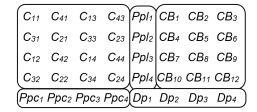
\includegraphics[scale=1]{figuras/phicc.PNG}
    \caption{Codificação do PHICC com 16 bits de entrada}{Fonte: \cite{magalhaes2019phicc}}
    \label{fig:phicc}
\end{figure}

Apesar de conseguir reduzir o custo da implementação, esse modelo acrescenta muitos bits e possui uma lógica de codificação complicada, podendo sobrecarregar a memória.      

\subsection{Técnicas de proteção para a CAM e TLB}

A abordagem de \cite{pagiamtzis2006soft} se utilizou da adição de um bit de paridade nos endereços para aumentar a distância Hamming entre endereços próximos. Este método servia para detectar bits com erros. Além disso, para melhorar a proteção contra erros, o esquema as técnicas de verificação do \textit{match line}. O método reduz a quantidade de erros nas células de memória sem acrescentar tempo de execução, mas adiciona área devido aos bits extras. A Figura \ref{fig:matchline} é uma representação desse esquema, onde pode ser vista a área adicionada referente à paridade. As células com D representam os bits armazenados e com P são os resultados das paridades de cada linha.

\begin{figure}[ht]
    \centering
    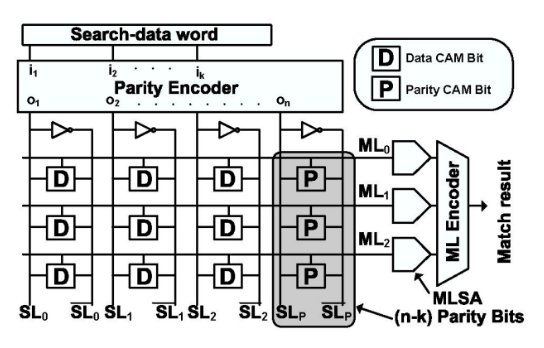
\includegraphics[scale = 0.7]{figuras/matchline.png}
    \caption{Esquema de proteção de CAM com paridade e aprimoramento do matchline}{Fonte: \cite{pagiamtzis2006soft}}
    \label{fig:matchline}
\end{figure}

Técnicas de redundância espacial foram utilizadas por \cite{lang2013processor} e \cite{maestro2013soft} para minimizar falhas nas células de memória. O primeiro usava uma cópia de \textit{back-up} com o conteúdo da TLB. Quando um erro era detectado, a TLB era simplesmente sobrescrita com a cópia. Já em \cite{maestro2013soft}, a técnica de duplicação era acompanhada por algoritmos capazes de detectar uma quantidade maior de erros, o que diminuía as falhas. Apesar disso, as duas técnicas duplicam o espaço de memória necessário para implementação.

Em \cite{sanchez2016combined}, os autores usam Hamming e paridade para implementar um código matricial SEC-DAED (do inglês, \textit{single error correction - double adjacent error detection}) que proteja CAMs e memórias associativas, como as TLBs. Protegendo sistemas de memória em geral, \cite{sanchez2012hamming} através da utilização de Hamming Estendido, implementa um código do tipo SEC-DED-TAED (do inglês, \textit{single error correction - double error detection - triple adjacent error detection}).

\cite{li2018efficient} propõe um código linear para tratar erros em TLBs, utilizando intercalação para codificar a palavra. O método se trata de dividir a palavra recebido em 4 grupos de bits e realizar cálculos de paridade entre esses grupos. Devido ao processo de intercalação, o código consegue tratar erros simples e duplo adjacentes. Além disso, no mesmo trabalho, os autores apresentam uma abordagem para minimizar a quantidade de bits de redundância em códigos para corrigir até erros quádruplos. Na Figura \ref{fig:4bit} está representada a lógica do circuito deste método, onde são avaliados diversos cenários com possibilidades de falhas em até 4bits. Na figura, cada "X" representa um bit com erro e "C" um bit correto. Por exemplo, XCXX possui uma configuração com um erro triplo, sendo que dois bits com erro são adjacentes. Comparado com outros métodos lineares, este acaba acrescentando ocupando muita área na implementação. 

\begin{figure}[ht]
    \centering
    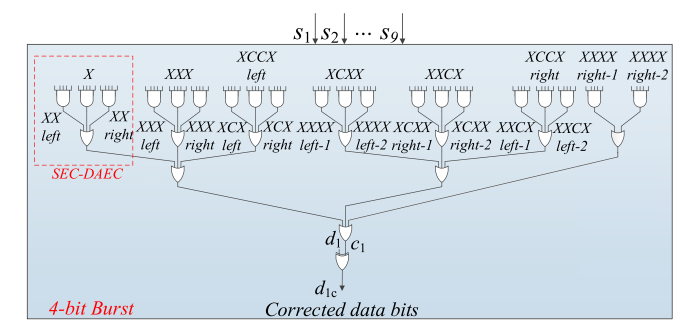
\includegraphics[scale=0.7]{modelo-dissertacao-ppgcc/figuras/4bitburst.PNG}
    \caption{Decodificação do código para  grupos de 4-bit de erros}{Fonte: \cite{li2018efficient}}
    \label{fig:4bit}
\end{figure}

Os autores de  \cite{kiani2019improving} apresentam um código em formato matricial com o objetivo de proteger TLBs contra falsos positivos. O esquema proposto também utiliza paridade para detectar e corrigir erros.  Na avaliação do código, foram analisados dois cenários: o primeiro reduz a capacidade de armazenamento da TLB para usar esse espaço para armazenar os bits de paridade, enquanto o segundo adiciona linhas e/ou colunas extras para fazer esta alocação. As taxas de correção são boas para erros simples e duplos, mas falham para erros triplos.

Uma abordagem focada na proteção de TLBs é apresentada em \cite{sanchez2019reducing}. Esse método será utilizado nos experimentos realizados neste trabalho, portanto ele será mais detalhado em uma seção própria, a seguir. 

\section{Paridade codificada nos NPVs}

O trabalho de \cite{sanchez2019reducing} propõe um método utilizado para diminuir a ocorrência de falsos positivos nas TLBs, aproveitando do conhecimento do princípio de localidade (ou localidade de referência). Sua abordagem trata da codificação dos números que representam as páginas virtuais (NPVs) de uma maneira específica antes que estes sejam armazenados nas TLBs. O método em questão foi implementado em um\textit{ Field Programmable Gate Array} (FPGA) e comparado com um esquema anterior, mostrando que ele pode fornecer melhor proteção para endereços vizinhos, sem custo adicional. A abordagem funciona bem, corrigindo até erros triplos adjacentes. 

Como pode ser visto na Figura \ref{fig:codeS}, o NPV é codificado e apresentado à TLB com a nova configuração. Neste método, não é necessário decodificar NPV’. Quando a CPU solicita um NPV, ele é codificado e a TLB tenta combiná-lo com os valores armazenados na CAM. Se houver o hit, o endereço físico será retornado. Se houver o miss, uma falha de página é emitida

\begin{figure}[ht]
    \centering
    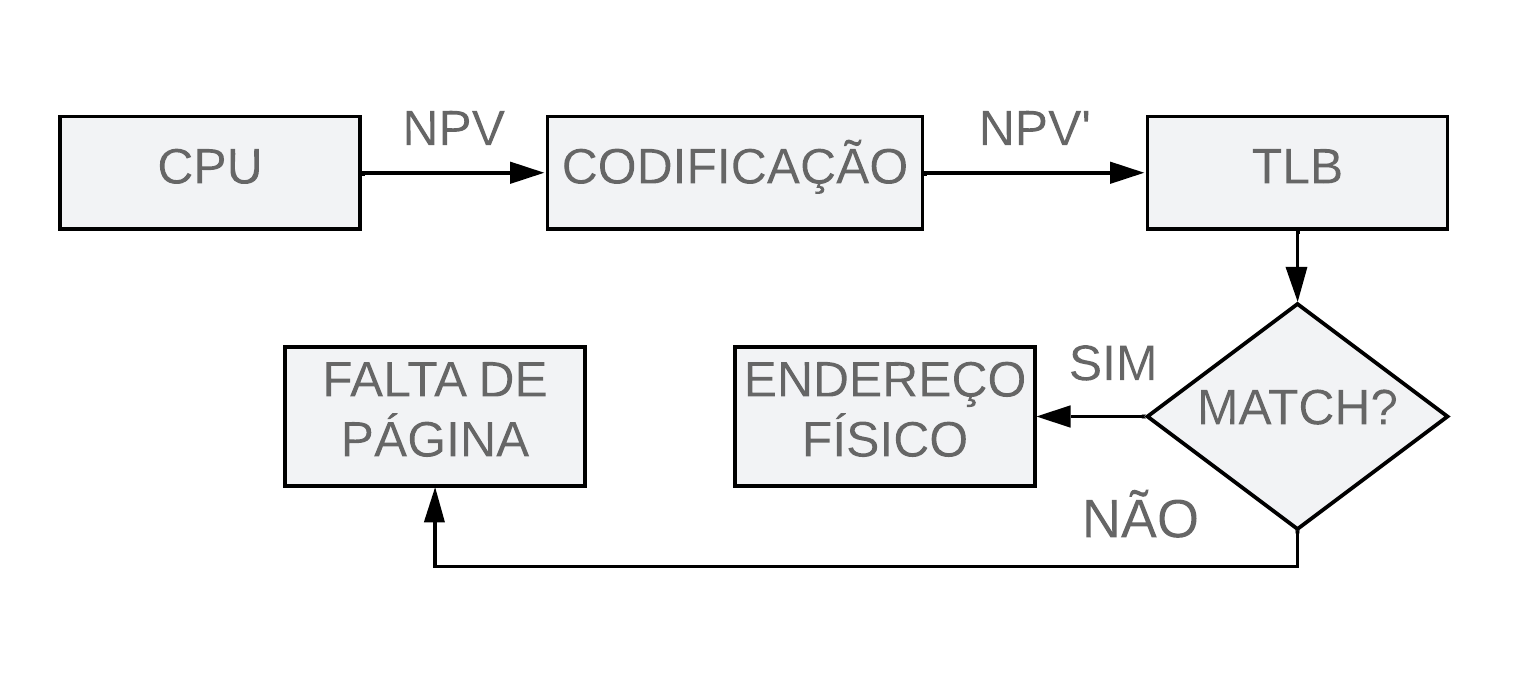
\includegraphics[scale=0.9]{figuras/match.png}
    \caption{Codificação e verificação de \textit{match}}{Fonte: próprio autor}
    \label{fig:codeS}
\end{figure}

A proposta do trabalho de \cite{sanchez2019reducing} era codificar os dois bits mais significativos (MSB, do inglês \textit{most significant bit}) de modo que sobrescrevesse nesses bits o resultado da paridade dos bits do NPV na TLB, alternando entre posições pares e ímpares, como mostrado a seguir.
\begin{equation}
    NPV'[MSB] = NPV[MSB] \oplus NPV[MSB-2] \oplus ... NPV[1]
\end{equation}
\begin{equation}
    NPV'[MSB-1] = NPV[MSB-1] \oplus NPV[MSB-3] \oplus ... NPV[0]
\end{equation}    
    

Os demais bits que não são os MSB ou o MSB-1 permanecem inalterados após a codificação. Na implementação física do esquema descrito, no cenário com um NPV de 32 bits, o circuito fica semelhante ao da Figura \ref{fig:32}. Uma porta XOR simples realiza a operação de paridade entre duas entradas, cada entrada desta representando um bit do NPV. Deste modo, são necessárias 30 portas XOR para chegar aos resultados das paridades que sobrescreverão os valores de MSB e MSB-1.

\begin{figure}[ht]
\centering
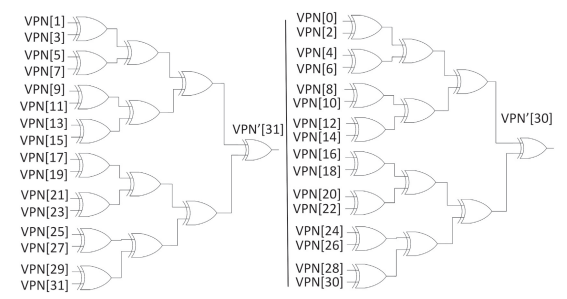
\includegraphics[scale=0.7]{figuras/32bit.png}
\caption{Circuito com as portas xor do cenário com 32 bits}{Fonte: \cite{sanchez2019reducing}}
\label{fig:32}
\end{figure}

Utilizando um exemplo de palavra com oito bits para simplificar a explicação: considere o NPV igual a 10100011. O bit mais significativo (MSB) é o bit 1 mais à esquerda, assim como o segundo bit mais significativo (MSB-1) é bit 0 à direita do MSB.

As equações para calcular o MSB e o MSB-1 a substituir os atuais ficam: 
\begin{equation}
   NPV'[MSB] = 1 \oplus 1 \oplus 0 \oplus 1    
\end{equation}
\begin{equation}
    NPV'[MSB-1] = 0 \oplus 0 \oplus 0 \oplus 1
\end{equation}
Nesse caso, o valor do MSB permanece 1, já que existe um número ímpar de bits 1, enquanto o MSB-1, pelo mesmo motivo, é convertido de 0 para 1. A nova palavra, o VPN', que será armazenada na TLB na mesma posição é 11100011.

A codificação por paridade nos NPVs incrementa a distância Hamming entre endereços vizinhos em dois bits. Isto garante que se as células de memória da TLB forem afetadas por um erro em um bit, nenhum \textit{single erorr} será produzido. Do mesmo modo, \textit{double adjacent errors} também são evitados, devido ao processo de calcular bits pares e ímpares separadamente.

\section{Conclusão}

A Tabela 1, a seguir, é um quadro comparativo com um resumo dos trabalhos relacionados citados anteriormente, apontando características da publicação e quais foram as abordagens e técnicas de codificação utilizadas em cada um. Percebe-se que paridade e Hamming são as técnicas de codificação mais utilizadas.

\begin{table}[ht]
\footnotesize
\centering
\caption{Quadro comparativo com resumo dos trabalhos relacionados}
\begin{tabular}{
>{\columncolor[HTML]{EFEFEF}}l |l|l|l}
\hline
\multicolumn{1}{c|}{\cellcolor[HTML]{EFEFEF}\textbf{\begin{tabular}[c]{@{}c@{}}Nome do\\ artigo\end{tabular}}} & \multicolumn{1}{c|}{\cellcolor[HTML]{EFEFEF}\textbf{\begin{tabular}[c]{@{}c@{}}Autores e ano de\\ publicação\end{tabular}}} & \multicolumn{1}{c|}{\cellcolor[HTML]{EFEFEF}\textbf{Abordagem}} & \multicolumn{1}{c}{\cellcolor[HTML]{EFEFEF}\textbf{\begin{tabular}[c]{@{}c@{}}Técnicas de\\ codificação\end{tabular}}} \\ \hline
\begin{tabular}[c]{@{}l@{}}CLC-A: An adaptive\\ implementation\\ of the Column\\ Line Code (CLC)\\ ECC\end{tabular} & \begin{tabular}[c]{@{}l@{}}Silva, Felipe et al.,\\ 2020\end{tabular} & Matricial. & \begin{tabular}[c]{@{}l@{}}Hamming Estendido e\\ paridade. Aprimora o\\ CLC padrão e o CLC\\ estendido\end{tabular} \\ \hline
\begin{tabular}[c]{@{}l@{}}PHICC: An error\\ correction code for\\ memory devices\end{tabular} & \begin{tabular}[c]{@{}l@{}}Magalhães et al.,\\ 2019\end{tabular} & Matricial. & \begin{tabular}[c]{@{}l@{}}Paridade, Hamming\\ e intercalação\end{tabular} \\ \hline
\begin{tabular}[c]{@{}l@{}}Reducing false\\ positives due to \\ double adjacent \\ errors in\\ instruction TLBs\end{tabular} & \begin{tabular}[c]{@{}l@{}}Sanchez-Mácian\\ et al., 2019\end{tabular} & \begin{tabular}[c]{@{}l@{}}Linear. Distancia\\ Hamming\end{tabular} & \begin{tabular}[c]{@{}l@{}}Paridade entre os bits,\\ alternando entre par e\\ ímpar, para armazenas\\ nos 2 MSBs\end{tabular} \\ \hline
\begin{tabular}[c]{@{}l@{}}Improving instruction\\ TLB reliability with\\ efficient multi-bit \\ soft error protection\end{tabular} & \begin{tabular}[c]{@{}l@{}}Kiani e Reviriego,\\ 2019\end{tabular} & Matricial. & \begin{tabular}[c]{@{}l@{}}Paridade vertical e\\ horizontal, alternando\\ entre par e ímpar. Uso\\ do espaço da TLB para\\ paridades\end{tabular} \\ \hline
\begin{tabular}[c]{@{}l@{}}Efficient\\ implementations of\\ 4-bit burst error\\ correction for\\ memories\end{tabular} & Li et al., 2018 & Linear & Intercalação e paridade \\ \hline
\begin{tabular}[c]{@{}l@{}}Combined modular\\ key and data error\\ protection for\\ content-addressable\\ memories\end{tabular} & \begin{tabular}[c]{@{}l@{}}Sanchez-Mácian,\\ Reviriego e\\ Maestro, 2016\end{tabular} & SEC-DAED & Hamming e paridade \\ \hline
\begin{tabular}[c]{@{}l@{}}Soft error tolerant\\ content-addressable\\ memories (cams)\\ using error detection\\ codes and duplication\end{tabular} & Maestro, 2013 & \begin{tabular}[c]{@{}l@{}}Redundância\\ espacial\end{tabular} & \begin{tabular}[c]{@{}l@{}}Duplicação da TLB e\\ algoritmo de detecção\end{tabular} \\ \hline
\begin{tabular}[c]{@{}l@{}}Processor fault \\ tolerance, through\\ translation lookaside\\ buffer refresh\end{tabular} & Lang, 2013 & \begin{tabular}[c]{@{}l@{}}Redundância\\ espacial\end{tabular} & \begin{tabular}[c]{@{}l@{}}Cópia da TLB e\\ atualização ao\\ encontrar erro\end{tabular} \\ \hline
\begin{tabular}[c]{@{}l@{}}A Hamming sec-daed\\ and extended\\ hamming sec-ded-taed\\ codes thtough\\ selective shortenning\\ and bit placement\end{tabular} & \begin{tabular}[c]{@{}l@{}}Sanchez-Mácian,\\ Reviriego e\\ Maestro, 2012\end{tabular} & \begin{tabular}[c]{@{}l@{}}SEC-DED-\\ TAED\end{tabular} & \begin{tabular}[c]{@{}l@{}}Hamming estendido\\ e paridade\end{tabular} \\ \hline
\begin{tabular}[c]{@{}l@{}}A soft-error toletant\\ content-addressable\\ memory (cam) using\\ an error-correction-\\ match-scheme\end{tabular} & \begin{tabular}[c]{@{}l@{}}Pagiamtzis, Azizi\\ e Najm, 2016\end{tabular} & \begin{tabular}[c]{@{}l@{}}Distancia \\ Hamming\end{tabular} & \begin{tabular}[c]{@{}l@{}}Aprimoramento do\\ match-line da CAM\end{tabular} \\ \hline
\end{tabular}
\end{table}

Com os conceitos apresentados neste capítulo, é possível entender com mais facilidade a proposta dessa pesquisa. O método exposto na seção 2.9 será explorado neste trabalho em outra abordagem, afim de obter resultados com menor custo de implementação. No próximo capítulo, serão mostrados a metodologia deste trabalho e detalhes dos experimentos realizados.

